% do not change these two lines (this is a hard requirement
% there is one exception: you might replace oneside by twoside in case you deliver 
% the printed version in the accordant format
\documentclass[11pt,titlepage,oneside,openany]{article}
\usepackage{times}


\usepackage{graphicx}
\usepackage{latexsym}
\usepackage{amsmath}
\usepackage{amssymb}
\usepackage{hyperref}

\usepackage{ntheorem}

% \usepackage{paralist}
\usepackage{tabularx}

% this packaes are useful for nice algorithms
\usepackage{algorithm}
\usepackage{algorithmic}

% well, when your work is concerned with definitions, proposition and so on, we suggest this
% feel free to add Corrolary, Theorem or whatever you need
\newtheorem{definition}{Definition}
\newtheorem{proposition}{Proposition}


% its always useful to have some shortcuts (some are specific for algorithms
% if you do not like your formating you can change it here (instead of scanning through the whole text)
\renewcommand{\algorithmiccomment}[1]{\ensuremath{\rhd} \textit{#1}}
\def\MYCALL#1#2{{\small\textsc{#1}}(\textup{#2})}
\def\MYSET#1{\scshape{#1}}
\def\MYAND{\textbf{ and }}
\def\MYOR{\textbf{ or }}
\def\MYNOT{\textbf{ not }}
\def\MYTHROW{\textbf{ throw }}
\def\MYBREAK{\textbf{break }}
\def\MYEXCEPT#1{\scshape{#1}}
\def\MYTO{\textbf{ to }}
\def\MYNIL{\textsc{Nil}}
\def\MYUNKNOWN{ unknown }
% simple stuff (not all of this is used in this examples thesis
\def\INT{{\mathcal I}} % interpretation
\def\ONT{{\mathcal O}} % ontology
\def\SEM{{\mathcal S}} % alignment semantic
\def\ALI{{\mathcal A}} % alignment
\def\USE{{\mathcal U}} % set of unsatisfiable entities
\def\CON{{\mathcal C}} % conflict set
\def\DIA{\Delta} % diagnosis
% mups and mips
\def\MUP{{\mathcal M}} % ontology
\def\MIP{{\mathcal M}} % ontology
% distributed and local entities
\newcommand{\cc}[2]{\mathit{#1}\hspace{-1pt} \# \hspace{-1pt} \mathit{#2}}
\newcommand{\cx}[1]{\mathit{#1}}
% complex stuff
\def\MER#1#2#3#4{#1 \cup_{#3}^{#2} #4} % merged ontology
\def\MUPALL#1#2#3#4#5{\textit{MUPS}_{#1}\left(#2, #3, #4, #5\right)} % the set of all mups for some concept
\def\MIPALL#1#2{\textit{MIPS}_{#1}\left(#2\right)} % the set of all mips





\begin{document}

\pagenumbering{roman}
% lets go for the title page, something like this should be okay
\begin{titlepage}
	\vspace*{2cm}
  \begin{center}
   {\Large Undirected Graphical Models\\}
   \vspace{2cm} 
   {Seminar - Artificial Intelligence\\}
   \vspace{2cm}
   {presented by\\
    David Hentschel \\
    Matriculation Number 1545724\\
   }
   \vspace{1cm} 
   {submitted to the\\
    Data and Web Science Group\\
    Melisachew W. \ Chekol\\
    University of Mannheim\\} \vspace{2cm}
   {Juli 2017}
  \end{center}
\end{titlepage} 

% no lets make some add some table of contents
% \tableofcontents
\newpage

%\listofalgorithms

%\listoffigures

%\listoftables

% evntuelly you might add something like this
% \listtheorems{definition}
% \listtheorems{proposition}

\newpage
% okay, start new numbering ... here is where it really starts
\pagenumbering{arabic}


\section{Introduction}
\label{sec:intro}
I will mainly refer to the insights described in \cite{koller2009probabilistic}.

Include (or understand) more of the main book \cite{koller2009probabilistic}. Partially Directed Models, Markov network independences parameterization revisited, bayesian networks and markov networks, summary and discussion

- what is a graphical mode?
 + a framework
 + as representation of (1) set of independencies and (2) sekleton for factorizing a distribution
 + a declarative representation that is a 'reasonable encoding of our world'
 + representation, inference, learning, see chapter 1.2.2

- short outline
 - first shot motivation why we want to do this and problem statement \ref{sec:motivation}
 - in section \ref{sec:methodology} first the essential fundamentals in form of the probability and graph theory as described, followed by how to represent a probabilistic model in a undirected graphical model, which leads to some selected possibilities of how inference and learning on those models works


\section{Motivation and Problem}
\label{sec:intro}
TODO:  Why is it important? What are the core challenges? How is this problem solved?

Directed probabilistic graphical models can represent many real-world problems. But there are some problems, which cannot be addressed by directed but by undirected graphical models. In addition to that undirected graphs might also be easier to understand and might represent a problem in an easier way.

A core advantage of undirected graphs for probabilistic modelling over for example a Baysian network (as common directed graphical model) is the property that undirected graphs are capable of representing cycles. For example if the impact of four planets on each other in terms of gravity should be modelled there is neither a starting nor a target point of dependency among those four planets. The acceleration of each planet mainly depends on the gravity fields of the three other planets (and the distance). Using undirected graphical models it is possible to represent such cyclic dependencies.

TODO: what more do we have?



\section{Methodology}
\label{sec:methodology}
\subsection{Essentials of probability theory and graph theory}
% 1.5 pages

\subsubsection{Probability theory}

The domain on probabilistic models is the probability theory. Probability describes how likely one beliefs that an event of uncertain nature occurs. By conducting multiple experiments or observing the behavior of a system, such probabilities can be estimated.

Because of the limited view onto a natural system, that humans or computers can have, probabilistic models are used to represent the main aspects of such system with uncertain events. Therefore a event space $\Omega$ is defined. $\Omega$ is a set of all possible outcomes of an event like rolling a die, $\Omega=\{1,2,3,4,5,6\}$.

In order to quantify the belief in how likely an outcomes emerges, a real number between zero and one, called probability, is assigned to each outcome, such that the sum of the probabilities of all outcomes is equal to one. This assignment is called probability distribution.

Upon random experiments random variables are defined, which might represent single possible outcomes of the event space or a more complex combination. They are used in order to formulate questions of inference. For example, how likely is it, that the sum of three dies is equal to four. The random variable $X$ hereby would be the sum of numbers on three dies after rolling them. The probability would be written as $P(X=4)$. Hereby $4$ is one value of $X$. The values of a random variable $X$ is often denoted as $x_1, x_2,  ..., x_n$, if there are n possible values.

Furthermore dependences or independences among random variables are important for inference. If it is known that one variable $A$ is independent from another variable $B$, it is not necessary to care about the $B$ when inferring about the probabilities of the values of $A$. $A$ is independent of $B$ if the probability distribution of $A$ does not change, whatever value $B$ attains.

In order to simplify probabilistic inference on large models, where we have a lot of random variables and dependencies, graphical models are used, as being discussed in sections \ref{sec:introugm} and the following.

\subsubsection{Graph theory} \label{sec:graph}

The second theoretical foundation of probabilistic graphical models is the graph theory. Graphs are used to represent and also illustrate a large variety of models, like also probabilistic models.

The basic components of a graph are a set of nodes and a set of edges, which represent relation between the nodes. In case of probabilistic models nodes represent random variables and edges represent the dependency between two random variables. An edge is a pair of nodes, which in the case of an directed edge needs to be ordered. If the graph is undirected the pairs of nodes have not necessarily to be ordered. This project paper mainly refers to undirected graphs.

Depending on the model graphs can be large and often only a restricted scope is needed to answer a certain question of interest. Therefore subgraphs are defined, such that the nodes of a subgraph is a subset of nodes of the original graph and the set of edges are all edges of the original graphs, whose nodes are also included in the subset of nodes. For example if their is a graph of relationships among students of an university and the question is how many relationships exists in a certain course, only the subgraph of the course is needed to answer the question. This might save computation time and space.

Furthermore a path from node $A$ to node $Z$ is a set of edges, such which connects those nodes $\{(A,B),(B,C),...,(Y,Z)\}$. If there is a path from one node to another in an undirected graphical model, those variables are at least indirectly dependent on each other.
% TODO: is that true???

If there is a path, where the starting point is the same as the end point without using an edge multiple times, this path is considered to by a cycle. As is described in section \ref{sec:bayes} Bayesian networks are not allowed to have cycles, whereas cycles can be represented in undirected graphical models.

\subsection{Introduction to undirected graphical model} \label{sec:introugm}
% 0.5 pages

\cite{hammersley1971markov}
\cite{pearl2014probabilistic}

As already described in section \ref{sec:graph}, in undirected graphical models nodes represent random variables and edges represent the dependences among those variables. Since the purpose of an undirected graphical model is to represent undirected mutual dependences between two variables at a time, the edges of the graph are also undirected. Probabilistic undirected graphical models are also called Markov networks or in some areas of application Markov random field, as is described in section \ref{sec:application}.

The following example, shown in figure \ref{fig:basic} (1) should illustrate a simple probabilistic model which is represented in a Markov network: Let there be four people $A$, $B$, $C$ and $D$, whereby it is unknown if their are vegetarian or not. Thus, their are four binary random variables. Furthermore it is known, that it is more likely that people that know each other are more likely to have the same eating habits than different ones. It is assumed that knowing people is mutual and not directed. As shown in figure \ref{fig:basic} (1) $C$ knows all, $D$ only knows $C$, $A$ knows $B$ and $C$ and $B$ knows $A$ and $C$. In order to infer new knowledge on this Markov network and actually calculate probabilities, the Markov network requires a quantification of affinities among the nodes, which will be discussed in the next section (\ref{sec:param}). In other words, how likely is it, that for example $A$ and $B$ both are vegetarian or that $A$ is vegetarian and $B$ is not. Figure \ref{fig:basic} (2) shows the graphical model of the misconception problem, which is described in \cite{koller2009probabilistic} (section 4.1). This second example is revisited in section \ref{sec:infer} in order to illustrate variable elimination as inference algorithm.

\begin{figure}[htpb]
  \centering
  	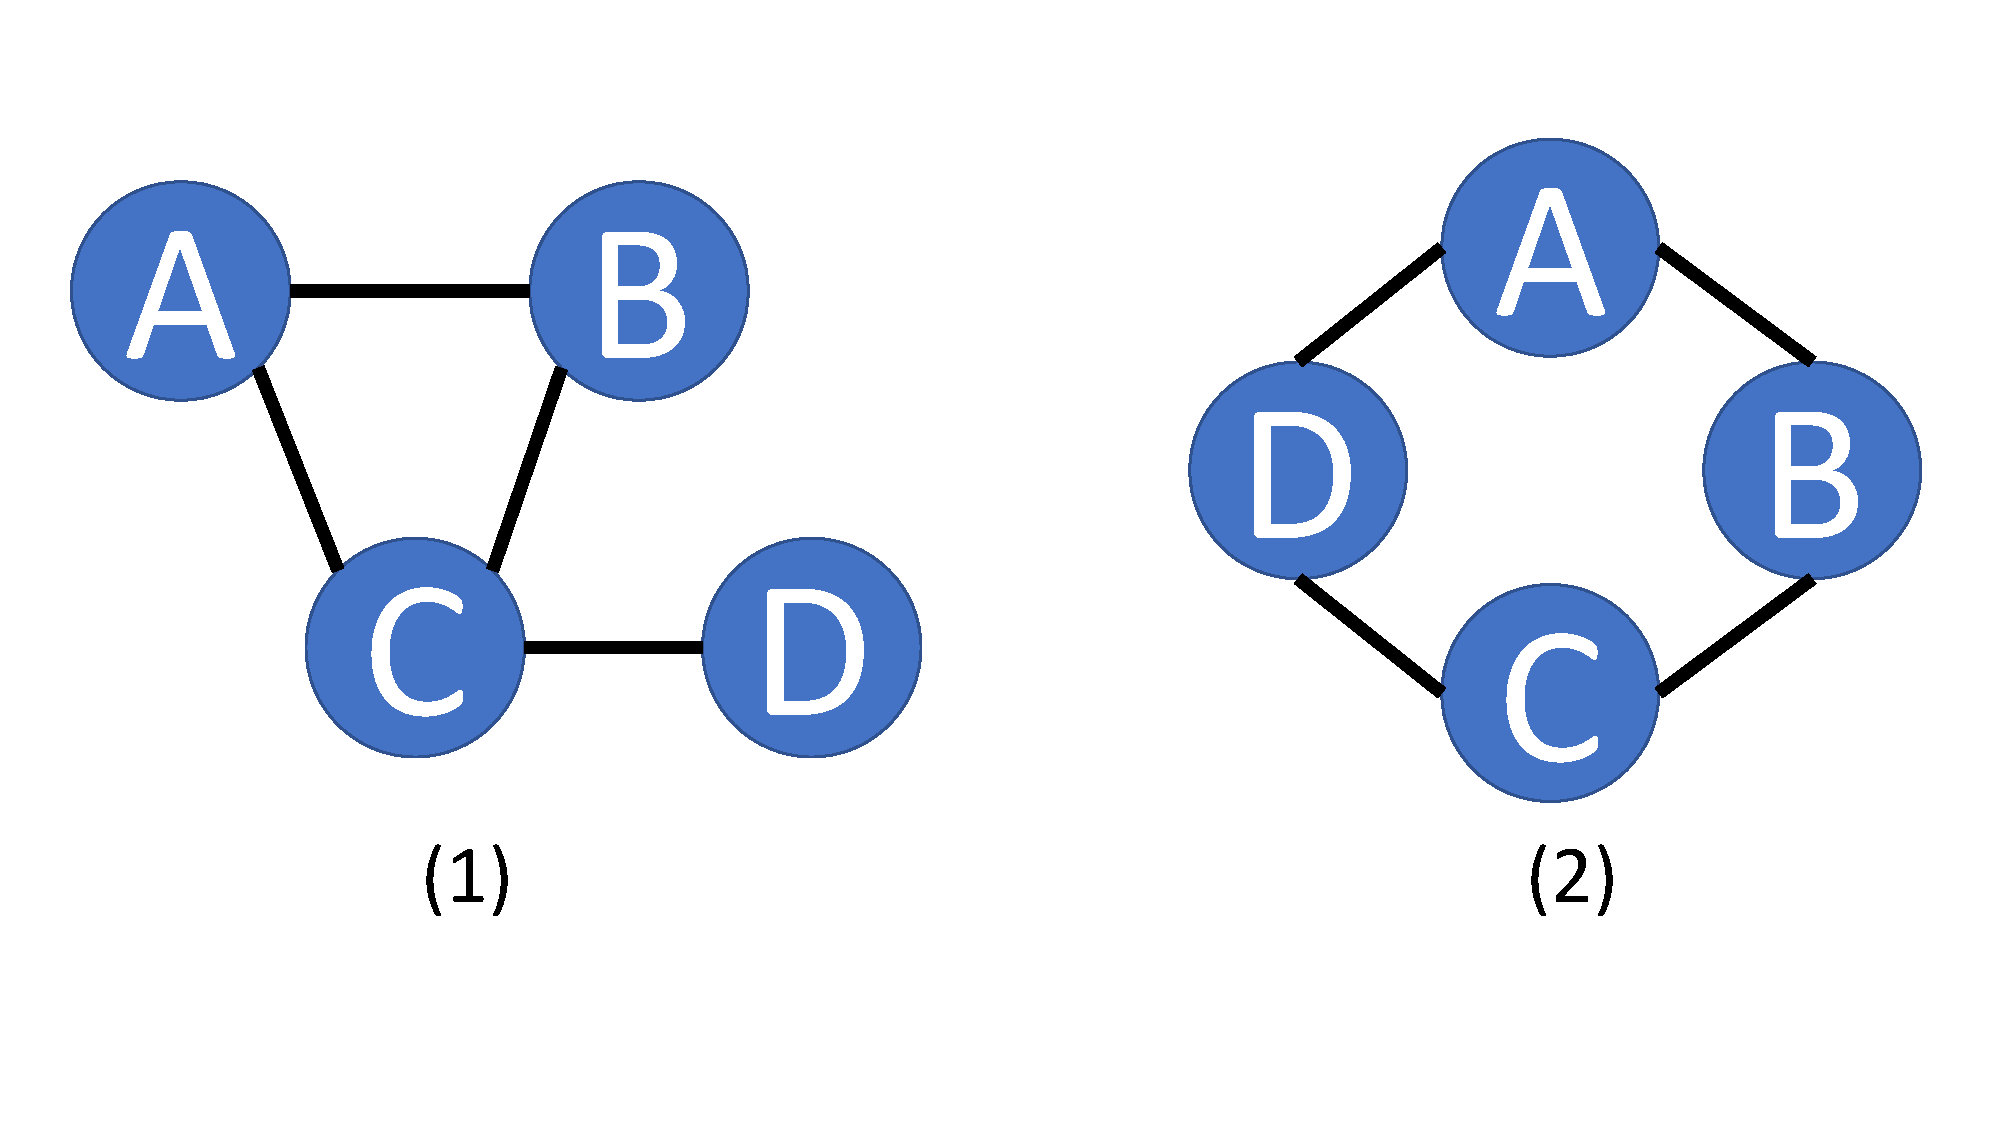
\includegraphics[scale=0.3]{img/basic.pdf} 
  \caption{Two simple examples of undirected graphical model}
  \label{fig:basic}
\end{figure}

\subsection{Parameterization} \label{sec:param}
% 2 pages

% TODO: short outlook into overparameterization

In order to conduct inference and learning on an Markov network, the model needs to be parameterized in the first place. Hereby the goal is to quantify the affinity, how likely the assignments of dependent variables are. The parameterization is achieved by assigning factors to subsets of random variables of the graph. The subsets needs to be cliques, which mean that each node in the clique depends on every other node in the clique. Each factor includes multiple parameters, which assign a real number to a certain combination of values of the random variable of the factors scope. For example, let $A$ and $B$ are binary random variables, which mutually depend on each other, their is a factor $\phi(A,B)$, which includes one parameter per assignment $\{(a_0,b_0),(a_0,b_1),(a_1,b_0),(a_1,b_1)\}$ . In contrary to the conditional probability distribution, which is used with Bayesian networks, as described in section \ref{sec:bayes}, the sum of assigned real numbers of a parameter do not necessarily need to sum up to one, because they do not directly represent probabilities but compatibilities amongst the nodes of the factor.

Figure \ref{fig:param} shows a factor of two dependent binary random variables and demonstrate the assignment of compatibility to each parameter.

\begin{figure}[htpb]
  \centering
  	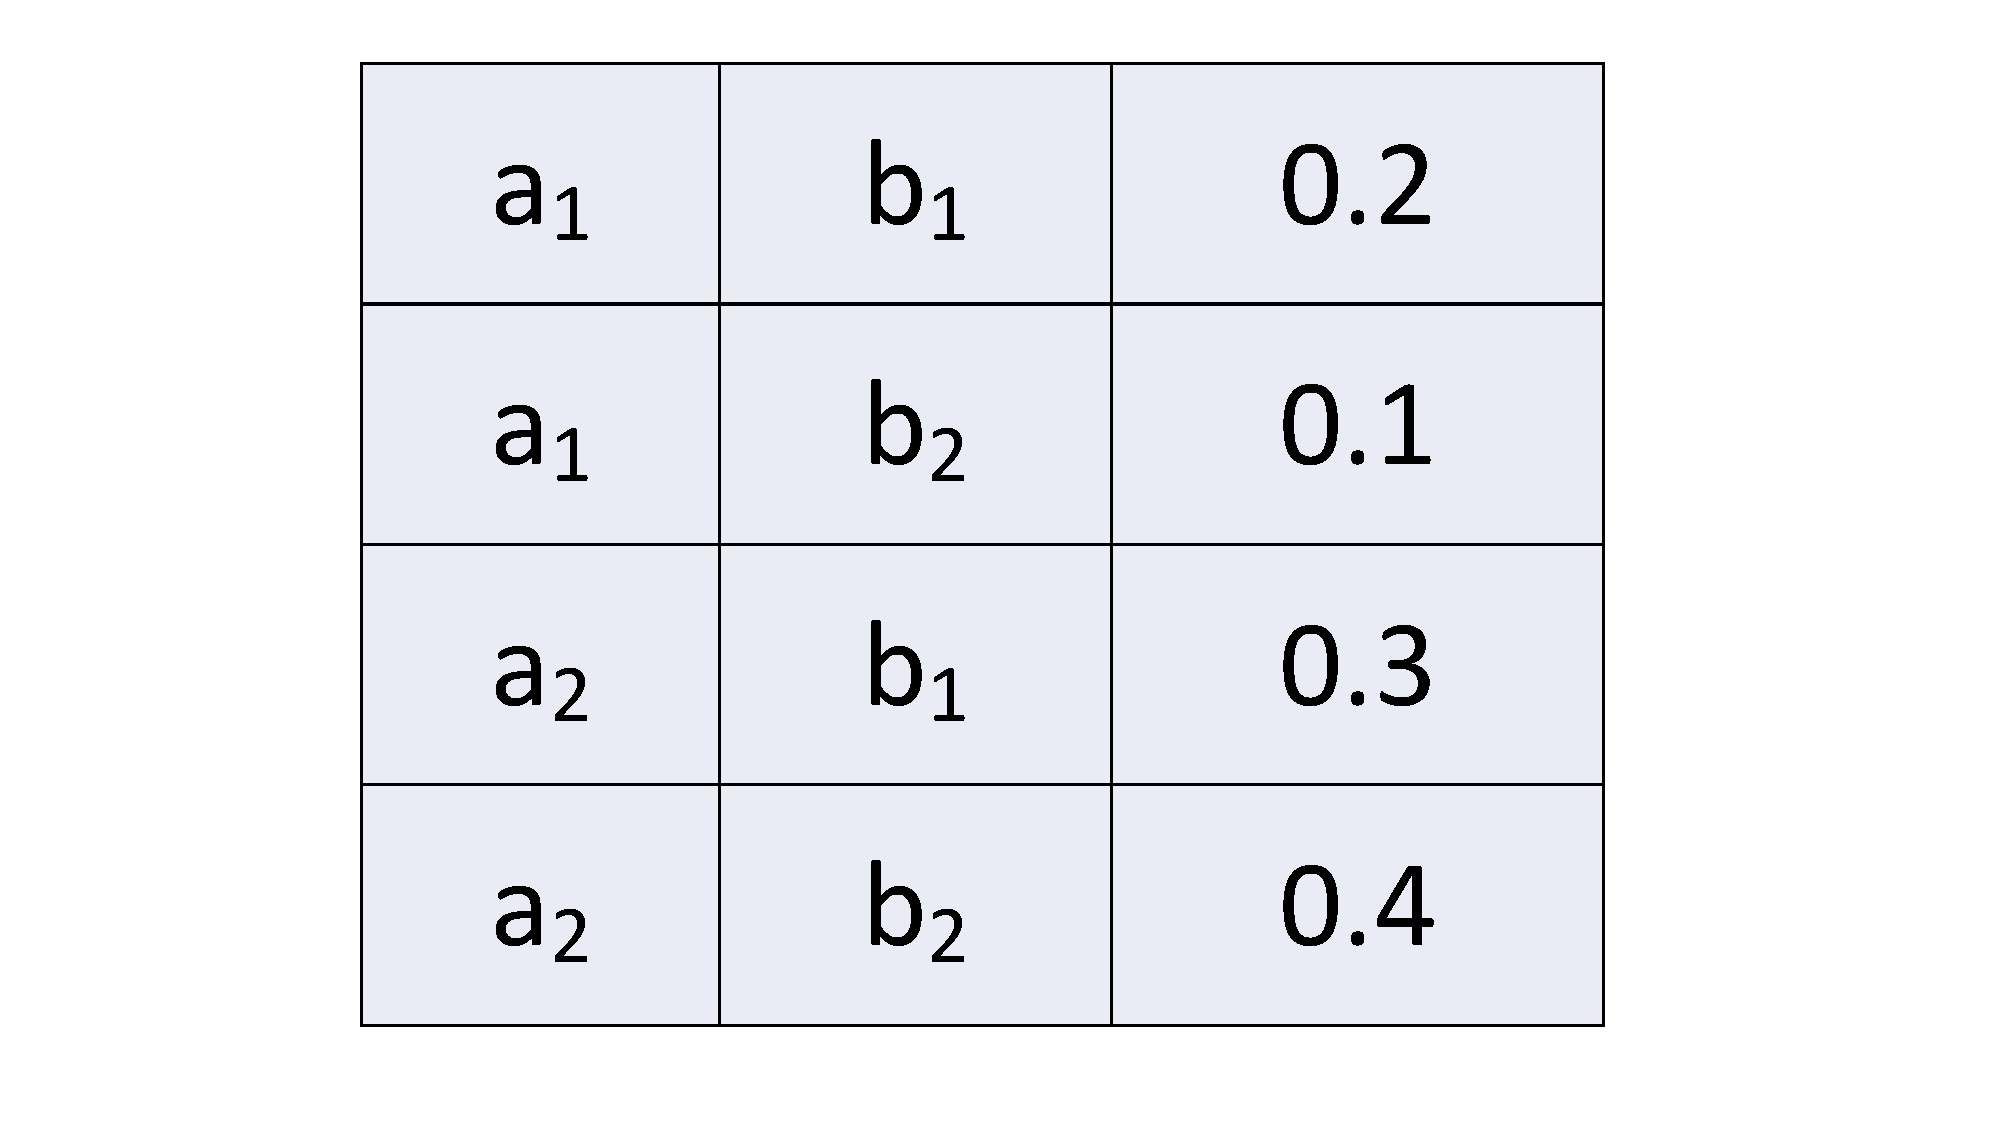
\includegraphics[scale=0.3]{img/param.pdf} 
  \caption{Factor of two binary linked random variables}
  \label{fig:param}
\end{figure}

In order to obtain the compatibility scores of assignments of all nodes, all factors are combined with a factor multiplication. Hereby the values of the parameters across the factors are multiplied in a way, that the assignments of the random variables match up. Thus, if $A$ and $B$ is one clique with $\Phi(A,B)$ and $B$ and $C$ is another clique with $\Phi(B,C)$, then $\Phi(A,B,C)=\Phi(A,B)\times\Phi(B,C)$. Figure \ref{fig:parammult} shows an example of a factor multiplication of factors with random variables. If all parameters are strictly positive than this distribution is also considered a Gibbs distribution, as described in \cite{kindermann1980markov}.

An important aspect of the resulting factor is that the number of parameters increased. While the two original factors $\Phi(A,B)$ and $\Phi(B,C)$ had in total ten parameters, the new factor $\Phi(A,B,C)$ contains twelve parameters. So if there are $n$ binary variables and each factor is defined on two variables, the number of parameters of the single factors would be $4\times n$ but the number of parameters of the factor product of all factors would be $2^n$, which leads to more computational space and time while processing a large model with many random variables. Section \ref{sec:indep} describes how independences and given values of random variables, help to reduce the scope of factor multiplications.

Besides the number of parameters the factor multiplication delivers also unnormalized compatibility scores and not probabilities. To achieve a probability distribution the scores needs to be normalized by the sum of all scores. How inference is possible with this probability distribution is discussed in section \ref{sec:infer}.

% TODO: image: use a,b,c like in the book and do unnormalized and normalized, like in the book

\begin{figure}[htpb]
  \centering
  	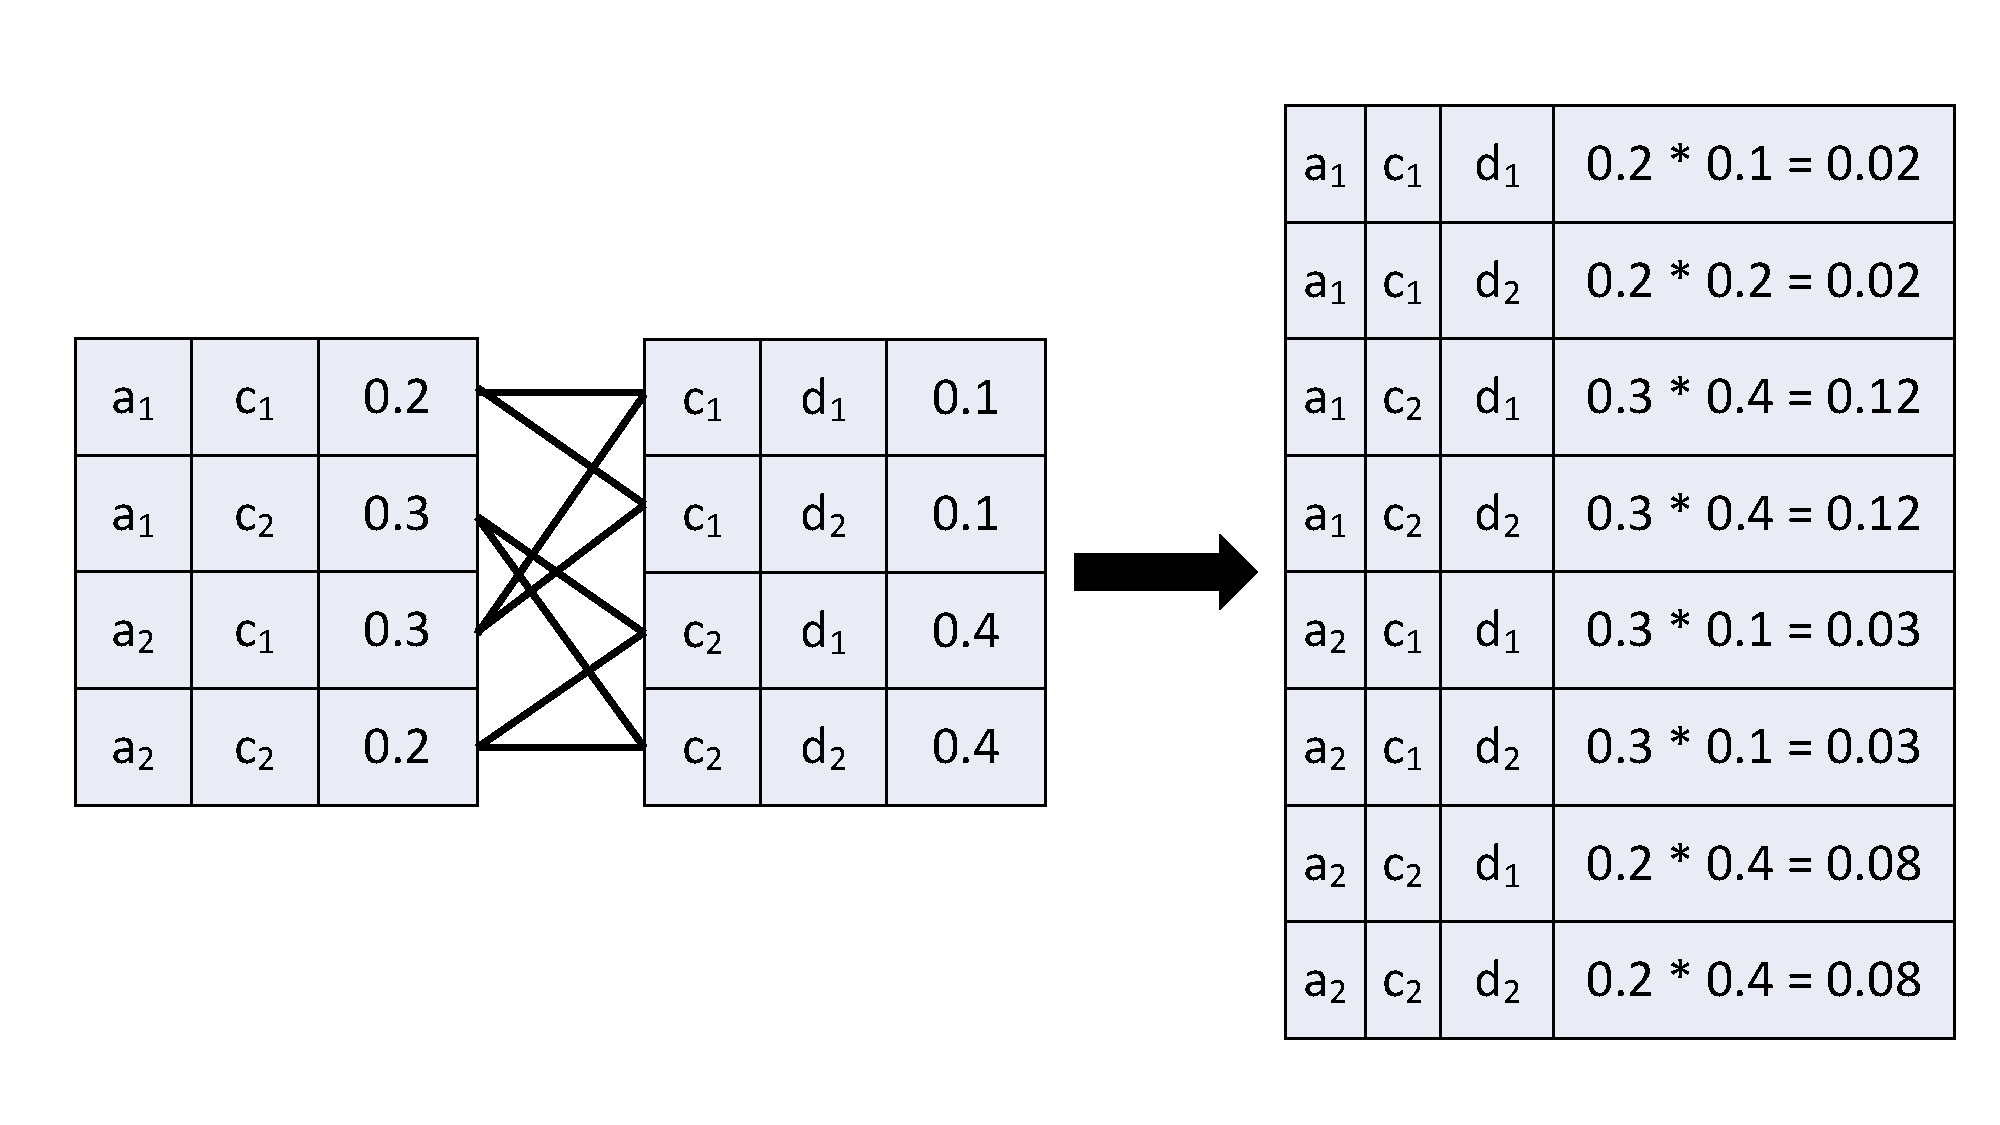
\includegraphics[scale=0.4]{img/parammult.pdf} 
  \caption{Factor multiplication of three binary random variables}
  \label{fig:parammult}
\end{figure}

In many applications alternative representations of factors are used to emphasize other aspects of the preferences among the values of variables. % TODO reference example sources
One alternative representation are log-linear models, which are for example used in Markov logic networks, as it is referred to in section \ref{sec:mln}. In log-linear models a factor is rewritten as $\phi(\mathbf{D}) = exp(-\epsilon(\mathbf{D}))$, where $\epsilon(\mathbf{D})=-ln\phi(\mathbf{D})$ is called the energy function. In general, a features is like a factor a function from $Val(\mathbf{D})$ to ${\rm I\!R}$. A special feature type is the indicator feature, which is often used to emphasize a certain value combination. If for example two variable $A_1$ and $A_2$ have the same set of values and the goal is to emphasize the assignment, in which both variables resolves in the same value, $\epsilon(A_1,A_2)$ can for those cases result in \textit{minus one} and otherwise in \textit{zero}. More in general the energy function is split into a product of a weight $w$ and the feature $f(\mathbf{D})$. This results in the representation of the unnormalized distribution shown in equation \ref{eq:loglin}. In contrast to the factor representation, the logarithmic representation might include multiple factors over the same set of variables. Especially in cases where the variables have large number of values, like when representing texts, the representation with indicator features can be beneficial. This property was for example utilized by Metzler and Croft to model term dependences in the context of information retrieval \cite{metzler2005markov}, which is further discussed in section \ref{sec:term}.

\begin{equation}
\widetilde{P}(D)=exp\left[-\sum_{i=k}^k{w_i f_i(\mathbf{D}_i)}\right]
\label{eq:loglin}
\end{equation}


\subsection{Independences in Markov networks} \label{sec:indep}
% 0.5 page

As described in section \ref{sec:introugm} the Markov network is supposed to represent the dependencies of a model. Since the dependencies are mutual, they flow along every direction through the graph, such that if there is a graph, in which there is a path from each node to every other node, all variables are indirectly dependent on each other, under the condition that their are no fixed assignments yet. In the contrary if there is a condition on a variables, the dependency "flow" stops right at this node.

From that the Markov properties are derived: the pairwise, local and global Markov property. The global Markov property states, that if there is a Markov network with a set of nodes $\mathbf{V}$ and two distinct subsets of nodes of $\mathbf{V}$ ($\mathbf{A}, \mathbf{B} \subset \mathbf{V} \wedge \mathbf{A} \cap \mathbf{B} = \emptyset$), and a third subset $\mathbf{C}$ that is also distinct from $\mathbf{A}$ and $\mathbf{B}$, the values of all its nodes are known and every path from a node of $\mathbf{A}$ to a node of $\mathbf{B}$ passes a node of $\mathbf{C}$, then all nodes of $\mathbf{A}$ are independent from all nodes of $\mathbf{B}$ and vise versa. This means, if there is a very large Markov network in practice and the need of inferring over a node, the computational effort in time and disc space can be dramatically reduced by finding such separating given subsets. This holds also for the local and the pairwise Markov property.

The local Markov property states, that if all adjacent nodes of a target node are given the target node is independent from all other nodes in the model. This set of adjacent nodes is also called Markov blanket and is also used in Bayesian networks, but with a different definition, as is described in section \ref{sec:bayes}. Finally the pairwise Markov property states, that two non-adjacent nodes are independent from each other, if all other nodes of the network are given. To be considered a Markov network the model needs to satisfy those three Markov properties, as described in \cite{markov1957theory}.


\subsection{Inference on undirected models} \label{sec:infer}
% 1 page

The goal of inference in probabilistic models is to gain knowledge like about unknown random variables. This section briefly discusses inferring knowledge about unknown variables, called query variables $Y$, given evidence $E=e$ in the form of known variables $P(Y|E=e)$ in Markov networks. Thus the result is a probability distribution over a set of query variables given a set of known variables. The set of query and the set of evidence variables are subsets of the set of all variables of the graph $Y,E \subset \mathcal{X}$.

Since the statement of the problem is of conditional nature, the definition of conditional probability can be applied:

\begin{equation}
P(\mathbf{Y}\ |\ E=e)=\frac{P(\mathbf{Y},e)}{P(e)}
\end{equation}

The probability $P(y,e)$ for a specific value $y \in Val(\mathbf{Y})$ can be computed by summing out all parameters of the full joint distribution where $y$ and $e$ matches the corresponding values in the distribution, as described in equation \ref{eq:sum}. Regarding Markov networks this would mean to sum out the normalized distribution.

\begin{equation}
P(y,e)=\sum_w{P(y,e,w)},\ with\ \mathbf{W} = \mathcal{X} - \mathbf{V} - \mathbf{E}
\label{eq:sum}
\end{equation}

In this context the independences, described in section \ref{sec:indep}, are useful in order to reduce the amount of factors, which are needed to compute the sufficient joint distribution. Thus, computational costs can be dramatically reduced, if the evidence cuts of large parts of the graph.

In any case, this approach is not efficient in terms of complexity. As described in section \ref{sec:param} the number of parameters in the full joint distribution increases exponentially with increasing random variables. To solve this problem algorithm were found, which either enable exact or approximated inference on Markov networks.

A simple algorithm for exact inference is variable elimination, which is in the following represented as one example of inference algorithms in Markov networks. As described above, in order to compute joint distribution all involved factors have to be multiplied and accordingly summed out. Equation \ref{eq:fullsum} shows the formula for computing the unnormalized distribution $\widetilde{P}(D)$ with respect to the graph, which was presented earlier in figure \ref{fig:basic} (2). Equation \ref{eq:rightsum} shows how the sum for $B$ is moved to the right and isolated all factors, which include the variable $B$. Based on this step the new factor $\tau_1(A,C)$ can be computed by applying the factor product and summing out $B$. Thus, the variable $B$ is eliminated from the calculation and replaced by the intermediate result $\tau_1(A,C)$, as can be seen in equation \ref{eq:reducedsum}. In the next steps also $A$ and $C$ are eliminated, so that the result is as in equation \ref{eq:endsum}. The resulting $\widetilde{P}(D)$ is proportional to $P(D)$ and can be mapped onto $P(D)$ by normalizing the score, as was described in section \ref{sec:param}.

\begin{equation}
\widetilde{P}(D)=\sum_A{\sum_B{\sum_C{\phi_1(A,B)\times\phi_2(B,C)\times\phi_3(C,D)\times\phi_4(A,D)}}}
\label{eq:fullsum}
\end{equation}

\begin{equation}
\widetilde{P}(D)=\sum_A{\sum_C{\phi_3(C,D)\times\phi_4(A,D)\times\sum_B{\phi_1(A,B)\times\phi_2(B,C)}}}
\label{eq:rightsum}
\end{equation}

\begin{equation}
\widetilde{P}(D)=\sum_A{\sum_C{\phi_3(C,D)\times\phi_4(A,D)\times\tau_1(A,C)}}
\label{eq:reducedsum}
\end{equation}

\begin{equation}
\widetilde{P}(D)=\tau_3(D)
\label{eq:endsum}
\end{equation}


Still the computation costs can be very high for exact inference, if the network is very large. In order to achieve viable computation times, approximation methods are used. Amongst them are for example the direct sampling or the Markov Chain Monte Carlo sampling. 
%TODO: cite sources (Short description)

%\subsection{Learning undirected models}
% 1 page

%\subsubsection{Motivation and Goals for learning probabilistic models}
% 0.5 pages
%- [chapter 16]
%- predictions, estimations

%\subsubsection{Likelihood function for learning}
% 0.5 pages

%- what is it
%- what methods, how does this satisfy the goals
%- specialty in comparison with Bayesian network
%- outlook


\section{Related Work}
\label{sec:relwork}
TODO: What other methods exist? What are the differences? What are the difficulties with other methods? How does it compare to a baseline method?

\href{https://www.math.leidenuniv.nl/scripties/BSC-Obbens.pdf}{Interisting stuff} \cite{obbens2014inference}


\subsection{Bayesian networks}
% 1 page

- chapter 3

TODO: probabilistic directed acyclic graphical model

TODO: \href{https://en.wikipedia.org/wiki/Bayesian_network}{wikipedia article}

TODO: image

TODO: Probabilistic reasoning in intelligent systems:Networks of Plausible Inference" written by Judea Pearl, chapter 3: Markov and Bayesian Networks:Two Graphical Representations of Probabilistic Knowledge, p.116:
The main weakness of Markov networks is their inability to represent induced and non-transitive dependencies; two independent variables will be directly connected by an edge, merely because some other variable depends on both. As a result, many useful independencies go unrepresented in the network. To overcome this deficiency, Bayesian networks use the richer language of directed graphs, where the directions of the arrows permit us to distinguish genuine dependencies from spurious dependencies induced by hypothetical observations.

\subsection{Partially directed models}
% 1 page

- chapter 4.6


\subsection{Markov logic network}
% 1 page

TODO: Classifying Topics and Detecting Topic Shifts in Political Manifestos with a Markov logic network \cite{zirn2016classifying}

TODO: probabilistic logic -> enabling uncertain inference

TODO: \href{https://en.wikipedia.org/wiki/Markov_logic_network}{wikipedia article}

TODO: \cite{koller2009probabilistic} chapter 20 learning undirected models

TODO: Main (first article about this) \cite{richardson2006markov}

TODO: application: Classifying Topics and Detecting Topic Shifts in Political Manifestos \cite{zirn2016classifying}

\subsection{Markov chain}
% optional: 1 page

TODO: Markov chain/ Markov process has time restrictions, Markov network has spatial restrictions

TODO: \href{https://en.wikipedia.org/wiki/Markov_chain}{wikipedia article}

TODO: image






\section{Application of Undirected Graphical Models}
\label{sec:application}
TODO: intro text
TODO: speech recognition

\subsection{Information retrieval: Term Dependencies}

TODO: forward and backward sources from this article \cite{metzler2005markov}
TODO: Get some more information from \url{http:\\www.slideplayer.com/slide/6012545}

Donald Metzler and W. Bruce Croft describe in \cite{metzler2005markov} a model for term dependencies using a Markov network. Afterwards this model can be used for information retrieval.

As in this article indicated every term of the query is considered as a random variable and are linked to the document which shall be ranked. In addition to this Metzler and Croft distinguish into three different dependecy assumptions: full independecy, sequential independency and full dependency among the terms as illustrated in \ref{fig:termdep}. Sequential dependency means that only ancient terms of the query are dependent like in a bigram model, full independency means that all query terms are conditionally independent from one another and finally full dependency describes a model, in which all query terms are coniditionally dependened on each other. 

In order to apply this method for a query following steps must be taken:
\begin{enumerate}
\item represent the query term dependencies by a Markov network
\item define potential functions for the cliques of the network
\item compute the rank of each document $P_\Lambda (D|Q)$ and sort them in a descending order
\end{enumerate}

\begin{figure}[htpb]
  \centering
  	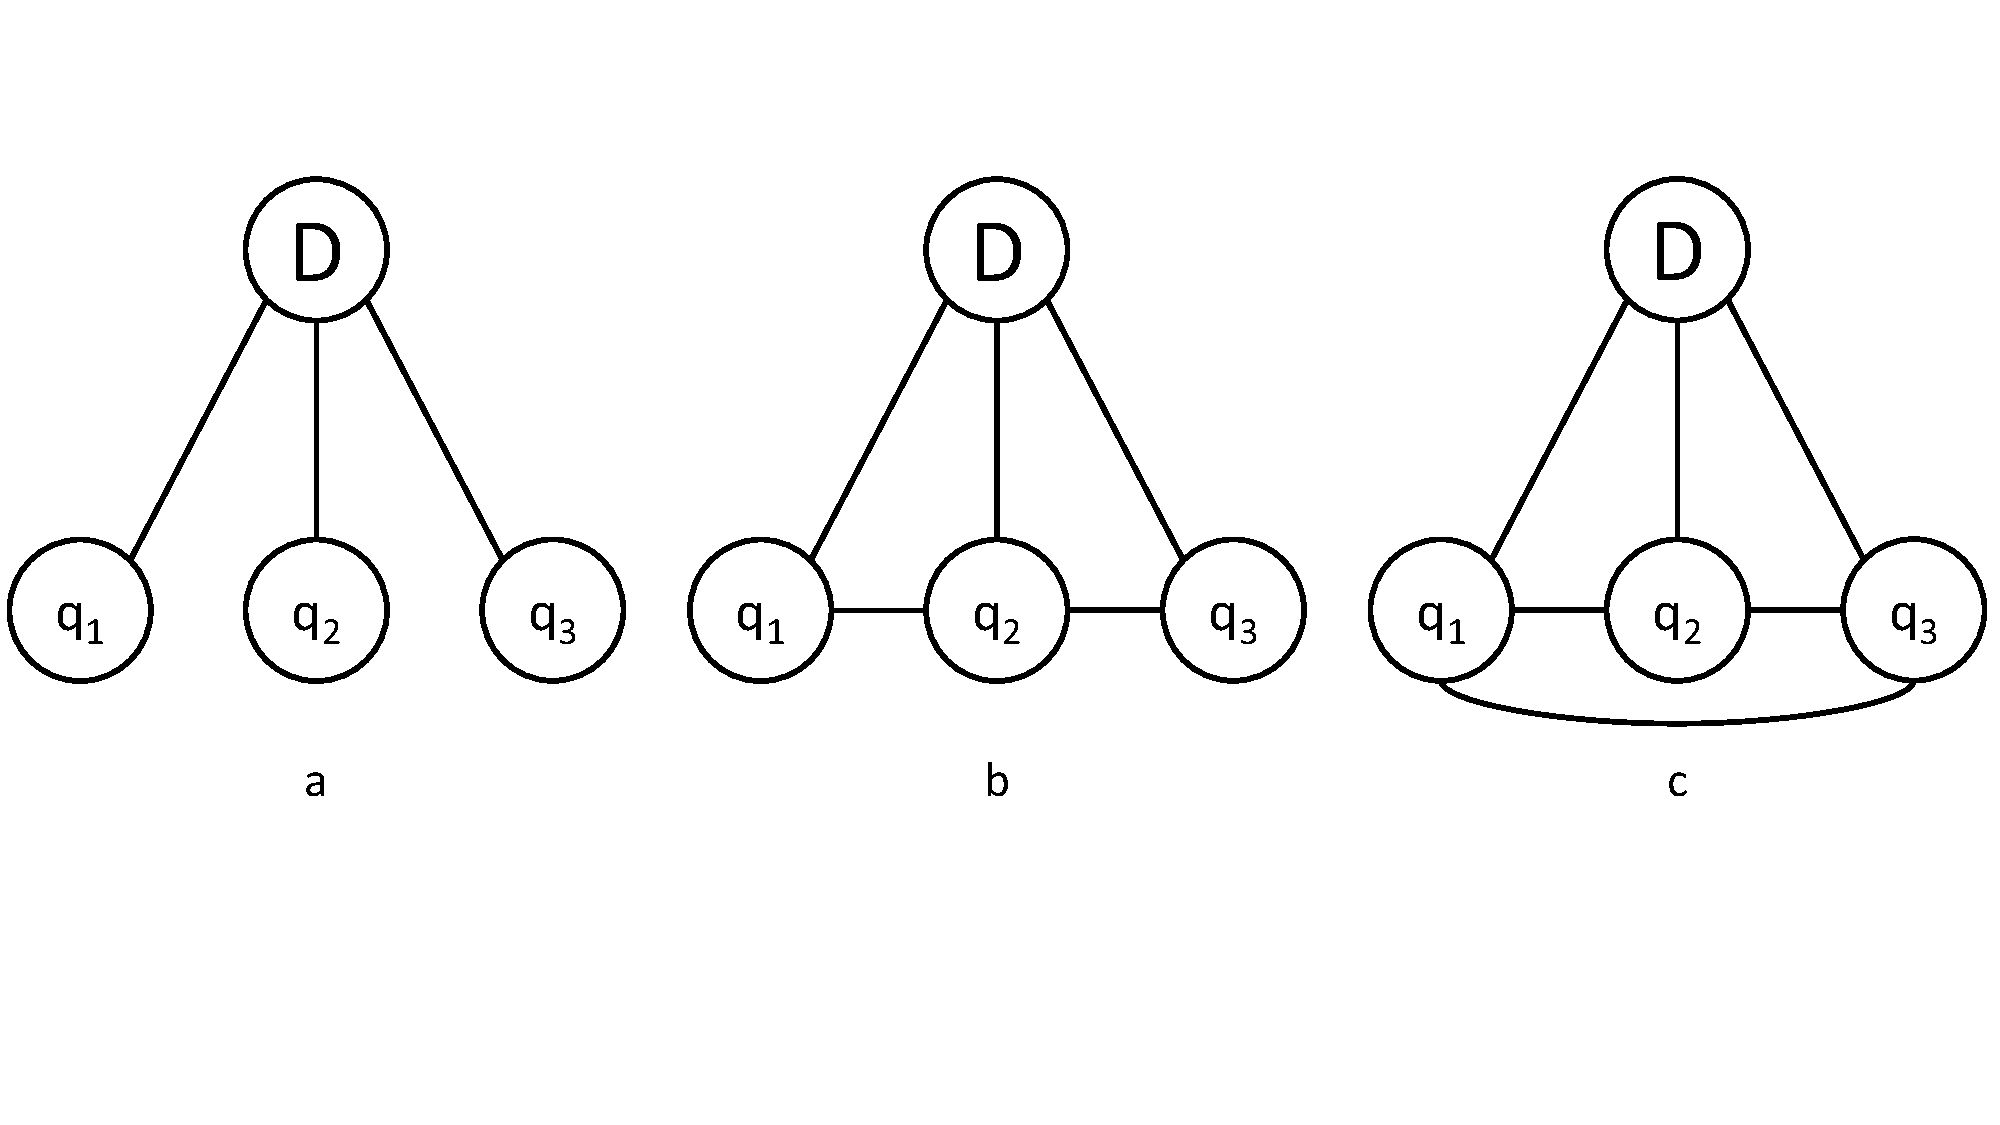
\includegraphics[scale=0.4]{img/termdep.pdf} 
  \caption{Dependency assumptions: a) full independency, b) sequential dependency and c) full dependency}
  \label{fig:termdep}
\end{figure}

Hereby D is a document, Q a query and $P_\Lambda$ a function which applies a weighted potential function to each clique of the Markov model. The potential functions can be considered as compatibility functions, as described in \ref{sec:methodology}, and are restriced to be strictly positive by \cite{metzler2005markov}. Further if full independency is assummed every term would form a smallest clique with the document under investigation and will lead to one contribution to the rank of the document with repect to the query. If elsewise full dependency is assummed, there are also cliques with all query terms and the document taken into account.

After experimenal testing on different data sets Metzler and Croft show the efficiency of this undirected graphical model approach in comparisson with other models like the bigram model. When comparing the three different independence assumptions the sequential dependecy assumption leads in terms of effectivity in contrast to the full independece assupmtion and also leads in terms of efficientcy and ad hoc requests in comparison with the full dependency assumption.


\subsection{Image processing Example: super-resolution}

TODO: figure wich shows the method, described below

One application of markov networks in the field of image processing is the computation of a super-resolution of an image. This means that a low-resolution image can be converted into an high-resoultion image, for instance by using an already trained example database, as described in \cite{freeman2002example}. As Freeman describes, first an training dataset is build by mapping a high resolution patch (for example 16 pxiels x 16 pixels) of any image to a low resolution counter patch (for example 8 pixels x 8 pixels) in order to use the reversed mapping later to find a high-resolution patch for a low-resolution input patch. Thus after training, there should be in the best case multiple high-resolution patches for one low-resolution patch.

In the next step an low-resolution input image is fragmented into multiple patches, which are represented by nodes in the Markov network. Furthermore the target high-resolution patches are also nodes which are at this point linked to the input nodes. To examine which high-resolution patch fits best, they overlap with their neighbor by one pixel. Thus, the best value combination of target patches needs to be minimized in terms of the error of the overlapping pixels or maximized in the terms of probability, how "likely" the resulting image fits to the input image.

\subsection{Machine learning: TODO}

TODO: write something about me



\section{Conclusion}
\label{sec:conclusion}
My conclusion is as follows


\bibliographystyle{plain}
\bibliography{seminar}

\end{document}

